\documentclass{standalone}
%outline around text
\usepackage[outline]{contour}
\contourlength{1.3pt}

%tikz
\usepackage{tikz}
\usetikzlibrary{knots, cd, calc}

\begin{document}


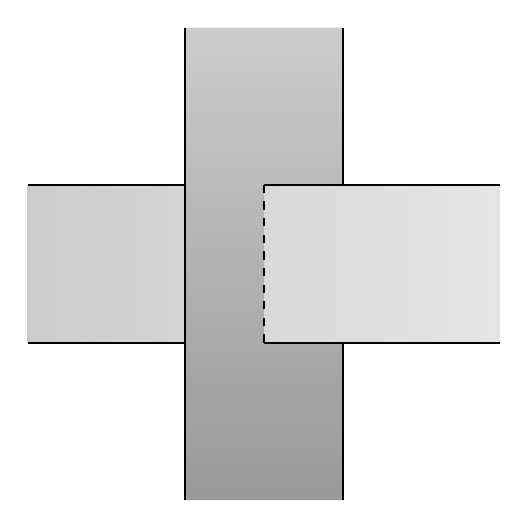
\begin{tikzpicture}
\clip (0, -2) rectangle (6, 4);
\shade[left color=black!20, right color = black!10] (0, 0) rectangle (6, 2);
\shade[bottom color=black!40, top color = black!20] (2, -2) -- (2, 4) -- (4, 4) -- (4, 2) -- (3, 2) -- (3, 0) -- (4, 0) -- (4, -2) -- (2, -2);
\draw[thick] (2, 0) -- (0, 0);
\draw[thick] (0, 2) -- (2, 2);
\draw[thick] (3, 2) -- (6, 2);
\draw[thick] (6, 0) -- (3, 0);
\draw[thick, dashed] (3, 0) -- (3, 2);
\draw[thick] (4, 2) -- (4, 4);
\draw[thick] (2, 4) -- (2, -2);
\draw[thick] (4, -2) -- (4, 0);
\end{tikzpicture}
\end{document}
